\documentclass[11pt,a4paper]{article}

\usepackage[margin=2.2cm]{geometry}
\usepackage{amsmath,amssymb,amsthm}
\usepackage{booktabs}
\usepackage{array}
\usepackage{tabularx}
\usepackage[shortlabels]{enumitem}
\usepackage{xcolor}
\usepackage{tikz}
\usepackage{fancyhdr}
\usepackage{setspace}
\usepackage{microtype}
\usepackage{titlesec}
\usepackage{hyperref}
\usepackage{listings}
\usepackage[skins,breakable]{tcolorbox}

\usetikzlibrary{positioning,arrows.meta,calc,fit,shapes.geometric,matrix,decorations.pathreplacing}

\definecolor{ink}{HTML}{222222}
\definecolor{rulegray}{HTML}{444444}
\definecolor{boxline}{HTML}{666666}
\definecolor{boxfill}{HTML}{F4F4F4}
\definecolor{boxtitle}{HTML}{E8E8E8}
\definecolor{g1}{HTML}{D0D0D0}
\definecolor{g2}{HTML}{9A9A9A}
\definecolor{g3}{HTML}{5A5A5A}

\hypersetup{
  colorlinks=true,
  linkcolor=black,
  urlcolor=black,
  pdftitle={MTL 458 Lecture 17: Concurrency: Locks},
  pdfauthor={Minati De, IIT Delhi}
}

\setstretch{1.12}
\raggedbottom
\setlist[itemize]{leftmargin=1.3em,itemsep=0.28em,topsep=0.35em}
\setlist[enumerate]{leftmargin=1.5em,itemsep=0.35em,topsep=0.4em}

\titleformat{\section}
  {\Large\bfseries\color{ink}}{\thesection.}{0.6em}{}
  [{\color{rulegray}\titlerule[0.5pt]}]
\titleformat{\subsection}
  {\large\bfseries\color{ink}}{\thesubsection}{0.55em}{}
\titleformat{\subsubsection}
  {\normalsize\bfseries\color{ink}}{\thesubsubsection}{0.5em}{}

\titlespacing*{\section}{0pt}{1.35em}{0.7em}
\titlespacing*{\subsection}{0pt}{1.05em}{0.45em}

\pagestyle{fancy}
\fancyhf{}
\renewcommand{\headrulewidth}{0.4pt}
\renewcommand{\footrulewidth}{0.3pt}
\fancyhead[L]{\small\color{ink}MTL 458 \textbullet\ Operating Systems}
\fancyhead[R]{\small\color{ink}Lecture 17: Concurrency: Locks}
\fancyfoot[C]{\small\thepage}
\setlength{\headheight}{14pt}

% ---------------------------------------------------------------------------
% Boxes
% ---------------------------------------------------------------------------
\tcbset{
  commonbox/.style={
    colback=boxfill, colframe=boxline, boxrule=0.5pt,
    left=6pt, right=6pt, top=5pt, bottom=5pt,
    fonttitle=\bfseries, coltitle=black, colbacktitle=boxtitle,
    enhanced, sharp corners=south, breakable
  }
}
\newtcolorbox{keybox}[1][]{commonbox, title={#1}}
\newtcolorbox{quizbox}[1][]{commonbox, title={#1}}
\newtcolorbox{solbox}[1][]{commonbox, title={#1}}
\newtcolorbox{warnbox}[1][]{commonbox, title={#1}}
\newtcolorbox{defbox}[1][]{commonbox, title={#1}}

\lstset{
  language=C,
  basicstyle=\ttfamily\small,
  keywordstyle=\bfseries,
  commentstyle=\itshape\color{g3},
  numbers=left, numberstyle=\scriptsize\color{g2}, numbersep=6pt,
  frame=single, rulecolor=\color{boxline},
  backgroundcolor=\color{boxfill},
  xleftmargin=1.6em, framexleftmargin=1.4em,
  columns=fullflexible, keepspaces=true,
  showstringspaces=false, breaklines=true,
  aboveskip=0.6em, belowskip=0.6em,
  morekeywords={bool,Boolean,Void,Typedef,lock_t,LockT,node_t,list_t,queue_t,pthread_mutex_t}
}
\lstdefinestyle{term}{language={}, numbers=none, basicstyle=\ttfamily\footnotesize,
  xleftmargin=0.4em, framexleftmargin=0.2em}

% Start a new page unless at least #1 of vertical space remains
\makeatletter
\newcommand{\keepspace}[1]{\par\penalty-100\begingroup
  \setlength{\dimen@}{#1}\dimen@ii\pagegoal\advance\dimen@ii-\pagetotal
  \ifdim\dimen@>\dimen@ii\ifdim\dimen@ii>\z@\vfil\fi\break\fi\endgroup}
\makeatother

% ---------------------------------------------------------------------------
% Timeline helpers (time axis 0..160; 1 unit = 0.075cm)
% ---------------------------------------------------------------------------
\tikzset{
  tl/.style={x=0.075cm, y=0.62cm, every node/.style={font=\scriptsize}},
  thA/.style={fill=black!70, draw=black},
  thB/.style={fill=black!10, draw=black},
  thC/.style={fill=black!45, draw=black},
  thD/.style={fill=black!25, draw=black}
}
% \blk{start}{end}{name}{style}{text colour}
\newcommand{\blk}[5]{\draw[#4] (#1,0) rectangle (#2,1);
  \node[text=#5, font=\scriptsize\bfseries] at ({(#1+#2)/2},0.5) {#3};}
% \ev{time}{label}: event label with a tick arrow down to the block
\newcommand{\ev}[2]{\node[font=\tiny, align=center, above] (e) at (#1,1.35) {#2};
  \draw[-{Latex[length=1.2mm]}] (#1,1.38) -- (#1,1.02);}
% \evhi{time}{label}: same, one row higher (for events close together)
\newcommand{\evhi}[2]{\node[font=\tiny, above] at (#1,1.95) {#2};
  \draw[-{Latex[length=1.2mm]}] (#1,1.98) -- (#1,1.02);}
% \spin{start}{end}: "spin" tag above a block
\newcommand{\spin}[2]{\node[font=\tiny, fill=black, text=white, inner sep=1.2pt] at ({(#1+#2)/2},1.22) {spin};}
\newcommand{\taxis}{\draw (0,-0.05) -- (160,-0.05);
  \foreach \t in {0,20,...,160} { \draw (\t,-0.05) -- (\t,-0.2); \node[below] at (\t,-0.15) {\t}; }}

\begin{document}

% ===========================================================================
% Title
% ===========================================================================
\begin{center}
{\color{rulegray}\rule{\textwidth}{1.1pt}}\\[0.45em]
{\LARGE\bfseries Operating Systems}\\[0.25em]
{\Large\bfseries MTL 458 \textperiodcentered\ Lecture 17}\\[0.35em]
{\LARGE\bfseries Concurrency: Locks}\\[0.35em]
{\large Minati De}\\[0.15em]
{\normalsize Department of Mathematics, Indian Institute of Technology Delhi}\\[0.35em]
{\color{rulegray}\rule{\textwidth}{1.1pt}}
\end{center}

\vspace{0.4em}
\begin{keybox}[Questions answered in this lecture]
\begin{itemize}
  \item Review: why threads, and why \textbf{mutual exclusion} for critical
        sections?
  \item How can locks be used to protect shared data structures such as
        \textbf{linked lists}?
  \item Can locks be implemented by \textbf{disabling interrupts}?
  \item Can locks be implemented with \textbf{loads and stores}?
  \item Can locks be implemented with \textbf{atomic hardware instructions}?
  \item When are \textbf{spinlocks} a good idea?
\end{itemize}
\end{keybox}

\tableofcontents
\vspace{0.6em}
\noindent{\color{rulegray}\rule{\textwidth}{0.4pt}}

% ===========================================================================
\section{Review: threads and correctness}
% ===========================================================================

\subsection{Which registers store the same / different values across threads?}

Two CPUs each run one thread of the same process. The slide's figure:

\begin{center}
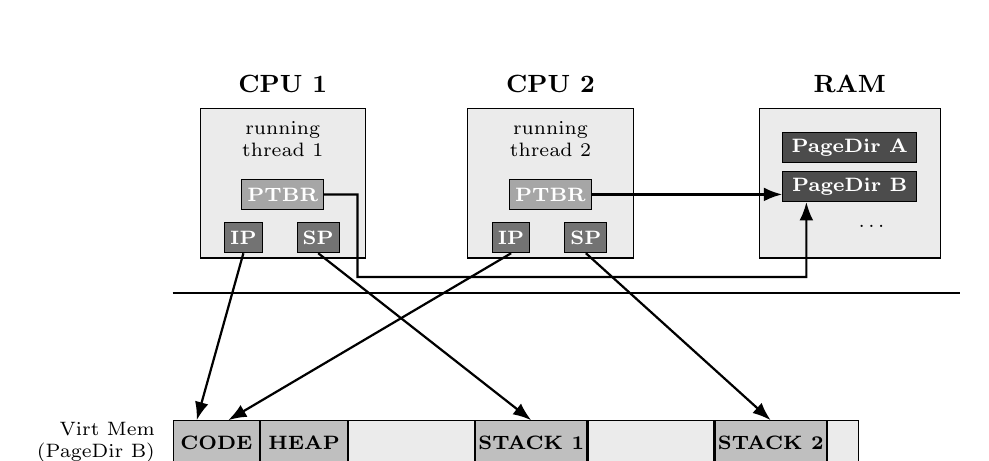
\begin{tikzpicture}[
  every node/.style={font=\small},
  cpu/.style={draw, fill=black!8, minimum width=2.1cm, minimum height=1.9cm, align=center, anchor=north},
  reg/.style={draw, fill=black!35, text=white, font=\scriptsize\bfseries, inner sep=2pt, minimum height=0.38cm},
  seg/.style={draw, minimum height=0.55cm, font=\scriptsize\bfseries, inner sep=1pt},
  arr/.style={-{Latex}, thick}
]
  \node[font=\small\bfseries] at (0,2.35) {CPU 1};
  \node[font=\small\bfseries] at (3.4,2.35) {CPU 2};
  \node[font=\small\bfseries] at (7.2,2.35) {RAM};
  \node[cpu] (c1) at (0,2.05) {};
  \node[cpu] (c2) at (3.4,2.05) {};
  \node[cpu, minimum width=2.3cm] (ram) at (7.2,2.05) {};
  \node[font=\scriptsize, align=center] at (0,1.65) {running\\thread 1};
  \node[font=\scriptsize, align=center] at (3.4,1.65) {running\\thread 2};
  \node[reg] (ptbr1) at (0,0.95) {PTBR};
  \node[reg] (ptbr2) at (3.4,0.95) {PTBR};
  \node[reg, fill=black!55] (ip1) at (-0.5,0.4) {IP};
  \node[reg, fill=black!55] (sp1) at (0.45,0.4) {SP};
  \node[reg, fill=black!55] (ip2) at (2.9,0.4) {IP};
  \node[reg, fill=black!55] (sp2) at (3.85,0.4) {SP};
  \node[reg, fill=black!70, minimum width=1.7cm] (pda) at (7.2,1.55) {PageDir A};
  \node[reg, fill=black!70, minimum width=1.7cm] (pdb) at (7.2,1.05) {PageDir B};
  \node[font=\scriptsize] at (7.5,0.55) {\ldots};
  \draw[thick] (-1.4,-0.3) -- (8.6,-0.3);

  \draw[arr] (ptbr1.east) -- (0.95,0.95) -- (0.95,-0.1) -- (6.65,-0.1)
        -- ($(pdb.south)+(-0.55,0)$);
  \draw[arr] (ptbr2.east) -- (pdb.west |- ptbr2.east);

  % virtual memory bar
  \node[font=\scriptsize, align=right, anchor=east] at (-1.5,-2.2) {Virt Mem\\(PageDir B)};
  \node[seg, fill=black!25, minimum width=1.1cm, anchor=west] (code) at (-1.4,-2.2) {CODE};
  \node[seg, fill=black!25, minimum width=1.1cm, right=0pt of code] (heap) {HEAP};
  \node[seg, fill=black!8, minimum width=1.6cm, right=0pt of heap] (g1) {};
  \node[seg, fill=black!25, minimum width=1.4cm, right=0pt of g1] (st1) {STACK 1};
  \node[seg, fill=black!8, minimum width=1.6cm, right=0pt of st1] (g2) {};
  \node[seg, fill=black!25, minimum width=1.4cm, right=0pt of g2] (st2) {STACK 2};
  \node[seg, fill=black!8, minimum width=0.4cm, right=0pt of st2] {};

  \draw[arr] (ip1.south) -- ($(code.north)+(-0.25,0)$);
  \draw[arr] (ip2.south) -- ($(code.north)+(0.15,0)$);
  \draw[arr] (sp1.south) -- (st1.north);
  \draw[arr] (sp2.south) -- (st2.north);
\end{tikzpicture}
\end{center}

\keepspace{9\baselineskip}
\begin{solbox}[Answer (second slide)]
\begin{itemize}
  \item \textbf{PTBR: same.} Both page-table base registers point to the
        same page directory (PageDir B): the threads share one address space.
  \item \textbf{IP: different.} Both instruction pointers point into the
        shared CODE, but at different instructions.
  \item \textbf{SP: different.} Each stack pointer points to that thread's
        own stack (STACK 1, STACK 2) in the shared address space.
\end{itemize}
\end{solbox}

\subsection{What is needed for correctness?}

\begin{center}
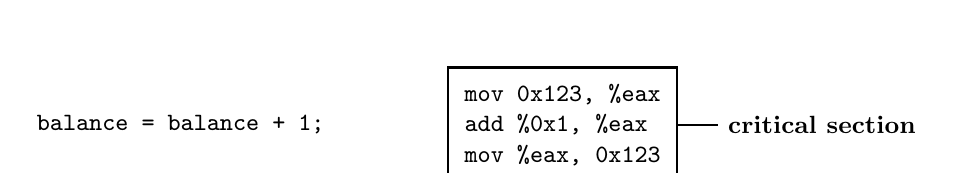
\begin{tikzpicture}
  \node[anchor=east, font=\ttfamily\small] at (-0.6,0) {balance = balance + 1;};
  \node[draw, thick, inner sep=6pt, align=left, font=\ttfamily\small] (cs) at (2.3,0) {
    mov 0x123, \%eax\\
    add \%0x1, \%eax\\
    mov \%eax, 0x123};
  \draw[thick] (cs.east) -- ++(0.5,0) node[right, font=\small] {\textbf{critical section}};
\end{tikzpicture}
\end{center}

Instructions accessing shared memory must execute as an
\textbf{uninterruptable group}: we need the instructions to be
\textbf{atomic}.

\begin{defbox}[More general: mutual exclusion]
We need \textbf{mutual exclusion} for critical sections: if thread A is in
the \textbf{critical section}, thread B can't be (it is okay if other
processes do unrelated work).
\end{defbox}

% ===========================================================================
\section{Other examples: a shared linked list}
% ===========================================================================

Multi-threaded applications do more than increment a shared balance.
Consider a multi-threaded application with a \textbf{shared linked list},
where all of these run concurrently:
\begin{itemize}
  \item Thread A inserting element \texttt{a},
  \item Thread B inserting element \texttt{b},
  \item Thread C looking up element \texttt{c}.
\end{itemize}

\begin{lstlisting}
typedef struct __node_t {
   int key;
   struct __node_t *next;
} node_t;

Typedef struct __list_t {
   node_t *head;
} list_t;

Void List_Init(list_t *L) {
   L->head = NULL;
}
\end{lstlisting}

\keepspace{19\baselineskip}
\begin{lstlisting}[firstnumber=13]
Void List_Insert(list_t *L, int key) {
   node_t *new = malloc(sizeof(node_t));
   assert(new);
   new->key = key;
   new->next = L->head;
   L->head = new;
}

int List_Lookup(list_t *L, int key) {
   node_t *tmp = L->head;
   while (tmp) {
      if (tmp->key == key)
         return 1;
      tmp = tmp->next;
   }
   return 0;
}
\end{lstlisting}

\texttt{List\_Insert} adds the new node at the \textbf{head}.
\texttt{List\_Lookup} walks the list and returns 1 if it finds \texttt{key}.

\begin{quizbox}[What can go wrong? Find a schedule that leads to a problem.]
Two threads insert at the same time.
\end{quizbox}

\subsection{Linked-list race}

\begin{center}
\renewcommand{\arraystretch}{1.15}
\begin{tabular}{@{}ll@{}}
  \toprule
  \textbf{Thread 1} & \textbf{Thread 2} \\
  \midrule
  \texttt{new->key = key} & \\
  \texttt{new->next = L->head} & \\
  & \texttt{new->key = key} \\
  & \texttt{new->next = L->head} \\
  & \texttt{L->head = new} \\
  \texttt{L->head = new} & \\
  \bottomrule
\end{tabular}
\end{center}

\textbf{Both entries point to the old head.} Only one entry can be the new
head: the one whose thread writes \texttt{L->head} \emph{last} (Thread 1
here).

\subsection{Resulting linked list}

\begin{center}
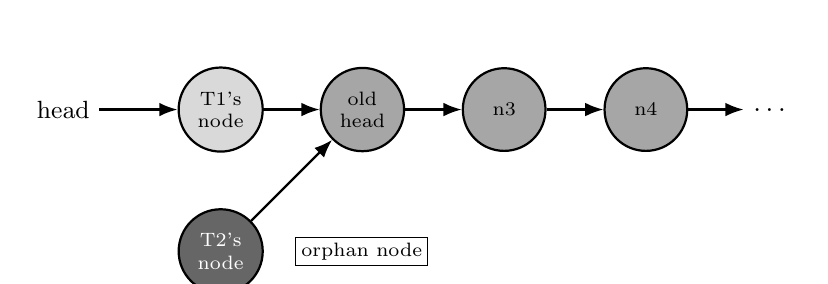
\begin{tikzpicture}[
  nd/.style={circle, draw, thick, minimum size=1.05cm, align=center, font=\scriptsize},
  arr/.style={-{Latex}, thick}]
  \node[font=\small] (h) at (0,0) {head};
  \node[nd, fill=black!15] (t1) at (2,0) {T1's\\node};
  \node[nd, fill=black!35] (oh) at (3.8,0) {old\\head};
  \node[nd, fill=black!35] (n3) at (5.6,0) {n3};
  \node[nd, fill=black!35] (n4) at (7.4,0) {n4};
  \node (dots) at (9,0) {\ldots};
  \node[nd, fill=black!60, text=white] (t2) at (2,-1.8) {T2's\\node};
  \node[font=\scriptsize, draw, inner sep=2pt, right=0.4cm of t2] {orphan node};
  \draw[arr] (h) -- (t1);
  \draw[arr] (t1) -- (oh);
  \draw[arr] (oh) -- (n3);
  \draw[arr] (n3) -- (n4);
  \draw[arr] (n4) -- (dots);
  \draw[arr] (t2) -- (oh);
\end{tikzpicture}
\end{center}

T2's node still points to the old head, but nothing points to T2's node: it
is an \textbf{orphan}, and key \texttt{b} is lost from the list.

% ===========================================================================
\section{Locking linked lists}
% ===========================================================================

\subsection{How to add locks?}

\textbf{One lock per list}: add a \texttt{pthread\_mutex\_t lock;} field to
the list and initialize it in \texttt{List\_Init}.

\begin{lstlisting}
Typedef struct __list_t {
   node_t *head;
   pthread_mutex_t lock;
} list_t;

Void List_Init(list_t *L) {
   L->head = NULL;
   pthread_mutex_init(&L->lock, NULL);
}
\end{lstlisting}

\keepspace{24\baselineskip}
\subsection{Approach \#1: consider everything a critical section}

\begin{lstlisting}
Void List_Insert(list_t *L, int key) {
   Pthread_mutex_lock(&L->lock);
   node_t *new = malloc(sizeof(node_t));
   assert(new);
   new->key = key;
   new->next = L->head;
   L->head = new;
   Pthread_mutex_unlock(&L->lock);
}

int List_Lookup(list_t *L, int key) {
   Pthread_mutex_lock(&L->lock);
   node_t *tmp = L->head;
   while (tmp) {
      if (tmp->key == key)
         return 1;
      tmp = tmp->next;
   }
   Pthread_mutex_unlock(&L->lock);
   return 0;
}
\end{lstlisting}

The whole body of both functions is the critical section. \textbf{Can the
critical section be smaller?}

\begin{warnbox}[Careful with early returns]
As drawn on the slides, \texttt{List\_Lookup} unlocks only before
\texttt{return 0}. The \texttt{return 1} path leaves with the lock still
held. A real implementation must unlock on \emph{every} return path.
\end{warnbox}

\keepspace{14\baselineskip}
\subsection{Approach \#2: critical section as small as possible}

\begin{lstlisting}
Void List_Insert(list_t *L, int key) {
   node_t *new = malloc(sizeof(node_t));
   assert(new);
   new->key = key;
   Pthread_mutex_lock(&L->lock);
   new->next = L->head;
   L->head = new;
   Pthread_mutex_unlock(&L->lock);
}
\end{lstlisting}

\texttt{malloc} and filling in \texttt{new->key} touch only the new,
still-private node, so they do not need the lock (assuming \texttt{malloc}
itself is thread-safe). Only the two lines that read and write the shared
\texttt{L->head} are critical. A bonus: if \texttt{malloc} fails, no lock
is held yet, whereas in Approach \#1 the failure path would also have to
unlock before returning.
\texttt{List\_Lookup} is locked exactly as in Approach \#1.

\subsection{Approach \#3: what about \texttt{Lookup()}?}

\texttt{List\_Insert} stays as in Approach \#2. For \texttt{List\_Lookup}
the slide notes:

\begin{keybox}[If there is no \texttt{List\_Delete()}, locks are not needed in \texttt{Lookup}]
Lookup only \emph{reads}. Insert fully builds the new node first and makes
it visible with the single store \texttt{L->head = new}. A concurrent lookup
sees either the old head or the new one, and every node it reaches is
complete and never freed. Only if nodes could be removed (and freed) while
a lookup is walking them would lookup need the lock.
\end{keybox}

% ===========================================================================
\section{Implementing synchronization}
% ===========================================================================

Build \textbf{higher-level synchronization primitives} in the OS:
operations that ensure correct ordering of instructions across threads.
\textbf{Motivation:} build them once and get them right.

\begin{center}
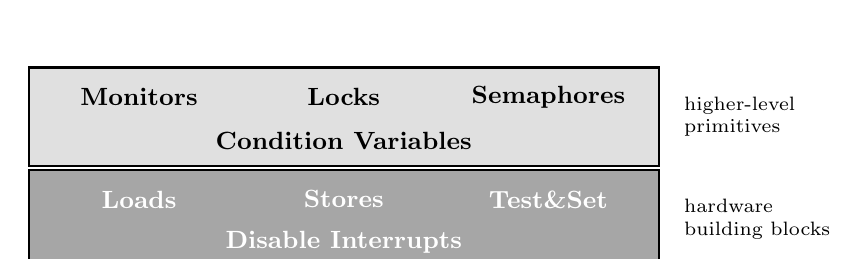
\begin{tikzpicture}[lay/.style={draw, thick, minimum width=8cm, minimum height=1.25cm}]
  \node[lay, fill=black!12] (top) at (0,1.3) {};
  \node[lay, fill=black!35] (bot) at (0,0) {};
  \node[font=\small\bfseries] at (-2.6,1.55) {Monitors};
  \node[font=\small\bfseries] at (0,1.55) {Locks};
  \node[font=\small\bfseries] at (2.6,1.55) {Semaphores};
  \node[font=\small\bfseries] at (0,1.0) {Condition Variables};
  \node[font=\small\bfseries, text=white] at (-2.6,0.25) {Loads};
  \node[font=\small\bfseries, text=white] at (0,0.25) {Stores};
  \node[font=\small\bfseries, text=white] at (2.6,0.25) {Test\&Set};
  \node[font=\small\bfseries, text=white] at (0,-0.3) {Disable Interrupts};
  \node[anchor=west, font=\scriptsize, align=left] at (4.2,1.3) {higher-level\\primitives};
  \node[anchor=west, font=\scriptsize, align=left] at (4.2,0) {hardware\\building blocks};
\end{tikzpicture}
\end{center}

The top layer (what programs use) is built from the bottom layer (what the
hardware provides). This lecture builds \textbf{locks}; the next lectures
build condition variables and semaphores.

\subsection{Lock implementation goals}

\begin{defbox}[Goals]
\textbf{Correctness}
\begin{itemize}
  \item \textbf{Mutual exclusion}: only one thread in the critical section
        at a time.
  \item \textbf{Progress} (deadlock-free): if several simultaneous
        requests, must allow one to proceed.
  \item \textbf{Bounded} (starvation-free): must eventually allow each
        waiting thread to enter.
\end{itemize}
\textbf{Fairness:} each thread waits for the same amount of time.

\textbf{Performance:} the CPU is not used unnecessarily (e.g.\ spinning).
\end{defbox}

Performance can be judged in three situations: no contention (one thread
locks and unlocks: what is the overhead?), several threads contending on
\emph{one} CPU, and threads contending from \emph{several} CPUs.

\subsection{Atomic operations}

To implement locks we need \textbf{atomic operations}.

\begin{defbox}[Atomic operation]
No other instructions can be \textbf{interleaved} with it.
\end{defbox}

Examples of atomic operations:
\begin{itemize}
  \item \textbf{Code between interrupts on uniprocessors}: disable timer
        interrupts, don't do any I/O.
  \item \textbf{Loads and stores of words}: \texttt{Load r1, B};
        \texttt{Store r1, A}.
  \item \textbf{Special hardware instructions}: \textbf{Test\&Set},
        \textbf{Compare\&Swap}.
\end{itemize}

The next sections try each of these in turn.

% ===========================================================================
\section{Implementing locks with interrupts}
% ===========================================================================

Turn off interrupts for critical sections:
\begin{itemize}
  \item this prevents the dispatcher from running another thread;
  \item so code between interrupts executes atomically.
\end{itemize}

\begin{lstlisting}
Void acquire(lockT *l) {
      disableInterrupts();
}

Void release(lockT *l) {
      enableInterrupts();
}
\end{lstlisting}

\begin{warnbox}[Disadvantages??]
\begin{itemize}
  \item \textbf{Only works on uniprocessors.} Disabling interrupts on one
        CPU does not stop a thread on another CPU from entering the
        critical section.
  \item \textbf{A process can keep control of the CPU for an arbitrary
        length} of time: a buggy or malicious program that disables
        interrupts and never re-enables them owns the machine.
  \item \textbf{Cannot perform other necessary work}: while interrupts are
        off, the OS misses timer and I/O interrupts.
\end{itemize}
Also, masking and unmasking interrupts is itself slow on modern CPUs.

Where it \emph{is} used: the OS itself sometimes disables interrupts briefly
to update its own data structures atomically. Inside the kernel the trust
problem disappears, since the OS trusts itself.
\end{warnbox}

\keepspace{20\baselineskip}
% ===========================================================================
\section{Implementing locks with loads and stores}
% ===========================================================================

\subsection{First attempt: one shared flag}

The code uses a single \textbf{shared} lock variable.

\begin{lstlisting}
Boolean lock = false; // shared variable

Void acquire(Boolean *lock) {
       while (*lock) /* wait */ ;
       *lock = true;
}

Void release(Boolean *lock) {
       *lock = false;
}
\end{lstlisting}

\keepspace{11\baselineskip}
\begin{quizbox}[Why doesn't this work? An example schedule that fails with 2 threads?]
\texttt{*lock == 0} initially.
\begin{center}
\renewcommand{\arraystretch}{1.12}
\begin{tabular}{@{}ll@{}}
  \toprule
  \textbf{Thread 1} & \textbf{Thread 2} \\
  \midrule
  \texttt{while(*lock == 1)} & \\
  & \texttt{while(*lock == 1)} \\
  & \texttt{*lock = 1} \\
  \texttt{*lock = 1} & \\
  \bottomrule
\end{tabular}
\end{center}
\end{quizbox}

\begin{warnbox}[Both threads grab the lock!]
Both threads see the lock free and both set it. \textbf{Problem: testing
the lock and setting the lock are not atomic.}

This schedule needs a context switch at exactly the wrong moment, which is
unlikely, but \emph{possible} is enough to show the lock is broken. Think
of the scheduler as malicious.
\end{warnbox}

\keepspace{16\baselineskip}
\subsection{Peterson's algorithm}

Assume only \textbf{two threads} (\texttt{tid} = 0, 1) and use \textbf{just
loads and stores}.

\begin{lstlisting}
int turn = 0; // shared
Boolean lock[2] = {false, false};

Void acquire() {
       lock[tid] = true;
       turn = 1-tid;
       while (lock[1-tid] && turn == 1-tid) /* wait */ ;
}

Void release() {
       lock[tid] = false;
}
\end{lstlisting}

\begin{itemize}
  \item \texttt{lock[tid] = true}: ``I want to enter.''
  \item \texttt{turn = 1-tid}: ``but you go first if you also want to.''
  \item Wait only while the \emph{other} thread wants in \emph{and} it is the
        other thread's turn.
\end{itemize}

\keepspace{14\baselineskip}
\subsection{Different cases}

Each table is one interleaving from the slides (Thread 0 left, Thread 1
right, time downward).

\begin{solbox}[Case 1: only thread 0 wants the lock]
\begin{center}
\begin{tabular}{@{}l@{}}
  \texttt{lock[0] = true;} \\
  \texttt{turn = 1;} \\
  \texttt{while (lock[1] \&\& turn == 1);} \\
\end{tabular}
\end{center}
\texttt{lock[1]} is false, so the loop exits at once: thread 0 enters.
\end{solbox}

\begin{solbox}[Case 2: both want the lock; thread 0 finishes its two stores first]
\begin{center}
\renewcommand{\arraystretch}{1.08}
\begin{tabular}{@{}ll@{}}
  \toprule
  \textbf{Thread 0} & \textbf{Thread 1} \\
  \midrule
  \texttt{lock[0] = true;} & \\
  \texttt{turn = 1;} & \\
  & \texttt{lock[1] = true;} \\
  & \texttt{turn = 0;} \\
  \texttt{while (lock[1] \&\& turn == 1);} & \\
  & \texttt{while (lock[0] \&\& turn == 0);} \\
  \bottomrule
\end{tabular}
\end{center}
\texttt{turn} ends as 0. Thread 0's test fails (\(\texttt{turn} \neq 1\))
so \textbf{thread 0 enters}; thread 1's test holds, so thread 1 spins.
\end{solbox}

\begin{solbox}[Case 3: both want the lock; thread 0 writes \texttt{turn} last]
\begin{center}
\renewcommand{\arraystretch}{1.08}
\begin{tabular}{@{}ll@{}}
  \toprule
  \textbf{Thread 0} & \textbf{Thread 1} \\
  \midrule
  \texttt{lock[0] = true;} & \\
  & \texttt{lock[1] = true;} \\
  & \texttt{turn = 0;} \\
  \texttt{turn = 1;} & \\
  \texttt{while (lock[1] \&\& turn == 1);} & \\
  & \texttt{while (lock[0] \&\& turn == 0);} \\
  \bottomrule
\end{tabular}
\end{center}
\texttt{turn} ends as 1. Thread 0 spins; thread 1's test fails, so
\textbf{thread 1 enters}.
\end{solbox}

\begin{solbox}[Case 4: both want the lock; thread 0 starts spinning early]
\begin{center}
\renewcommand{\arraystretch}{1.08}
\begin{tabular}{@{}ll@{}}
  \toprule
  \textbf{Thread 0} & \textbf{Thread 1} \\
  \midrule
  \texttt{lock[0] = true;} & \\
  \texttt{turn = 1;} & \\
  & \texttt{lock[1] = true;} \\
  \texttt{while (lock[1] \&\& turn == 1);} & \\
  & \texttt{turn = 0;} \\
  & \texttt{while (lock[0] \&\& turn == 0);} \\
  \texttt{while (lock[1] \&\& turn == 1);} & \\
  \bottomrule
\end{tabular}
\end{center}
At first thread 0 spins (\texttt{lock[1]} true, \texttt{turn} = 1). Then
thread 1 sets \texttt{turn = 0} and itself spins. Thread 0's next check
fails (\(\texttt{turn} = 0\)), so \textbf{thread 0 enters}.
\end{solbox}

\begin{keybox}[Pattern]
When both threads want the lock, the thread that writes \texttt{turn}
\textbf{last} waits; the other one enters. \texttt{turn} has one value, so
exactly one of them enters.
\end{keybox}

\keepspace{16\baselineskip}
\subsection{Peterson's algorithm: intuition}

\begin{itemize}
  \item \textbf{Mutual exclusion:} enter the critical section if and only if
    \begin{itemize}
      \item the other thread does not want to enter, or
      \item the other thread wants to enter, but it is your turn.
    \end{itemize}
  \item \textbf{Progress:} both threads cannot wait forever at the
        \texttt{while()} loop:
    \begin{itemize}
      \item it completes if the other process does not want to enter;
      \item otherwise the other process (the one matching \texttt{turn})
            will eventually finish.
    \end{itemize}
  \item \textbf{Bounded waiting} (not shown in the examples): each process
        waits at most one critical section. After the other thread leaves
        and tries again, it sets \texttt{turn} to you and must wait.
\end{itemize}

\begin{warnbox}[Peterson in practice]
Peterson's algorithm shows that a lock \emph{can} be built from loads and
stores alone. Real systems use hardware atomic instructions instead.
Algorithms like this do not work on modern hardware anyway: CPUs may
reorder loads and stores (relaxed memory consistency), so the
interleavings above are not the only possible ones.
\end{warnbox}

% ===========================================================================
\section{Locks with atomic hardware instructions}
% ===========================================================================

\subsection{\texttt{xchg}: atomic exchange, or test-and-set}

\begin{lstlisting}
// xchg(int *addr, int newval)
// return what was pointed to by addr
// at the same time, store newval into addr

int xchg(int *addr, int newval) {
  int old = *addr;
  *addr = newval;
  return old;
}
\end{lstlisting}

The C code only describes the behaviour: the hardware does the read and the
write as \textbf{one atomic instruction}.

\subsection{Lock implementation with \texttt{xchg}}

The slide first leaves blanks (\texttt{??}, \texttt{????}) and then fills
them in:

\begin{lstlisting}
typedef struct __lock_t {
  int flag;
} lock_t;

void init(lock_t *lock) {
  lock->flag = 0;
}

void acquire(lock_t *lock) {
  while(xchg(&lock->flag, 1) == 1) ;
  // spin-wait (do nothing)
}

void release(lock_t *lock) {
  lock->flag = 0;
}
\end{lstlisting}

\begin{keybox}[Why this works]
\texttt{flag} = 0 means free, 1 means held. \texttt{xchg(\&flag, 1)}
always writes 1 and returns the old value:
\begin{itemize}
  \item old value 0: the lock was free and \emph{we} just took it: exit the
        loop.
  \item old value 1: someone else holds it; writing 1 again changes nothing:
        keep spinning.
\end{itemize}
Testing and setting now happen in one atomic step, which fixes the
load/store race.

On a \emph{single} CPU, a spinlock needs a \textbf{preemptive} scheduler (a
timer interrupt). Otherwise the spinning thread never gives up the CPU and
the holder never runs to release the lock.
\end{keybox}

\keepspace{18\baselineskip}
\subsection{Other atomic hardware instructions: compare-and-swap}

\begin{lstlisting}
int CompareAndSwap(int *addr, int expected, int new) {
  int actual = *addr;
  if (actual == expected)
    *addr = new;
  return actual;
}

void acquire(lock_t *lock) {
  while(CompareAndSwap(&lock->flag, 0, 1)
          == 1) ;
  // spin-wait (do nothing)
}
\end{lstlisting}

The slide asks for the \texttt{?}s in
\texttt{CompareAndSwap(\&lock->flag, ?, ?) == ?}; the answer is
\texttt{0, 1} and \texttt{== 1}: ``if the flag is 0 (free), set it to 1;
keep spinning while the old value was 1.'' (The second version of the slide
names the first parameter \texttt{ptr} but the body still uses
\texttt{addr}; they are the same pointer.)

% ===========================================================================
\keepspace{16\baselineskip}
\section{Fairness}
% ===========================================================================

Going back to the lock goals with the emphasis now on \textbf{fairness}:
each thread should wait for the same amount of time.

\subsection{Basic spinlocks are unfair}

\begin{center}
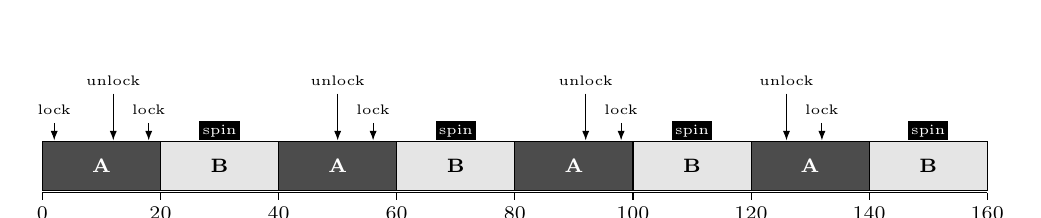
\begin{tikzpicture}[tl]
  \blk{0}{20}{A}{thA}{white}   \blk{20}{40}{B}{thB}{black}
  \blk{40}{60}{A}{thA}{white}  \blk{60}{80}{B}{thB}{black}
  \blk{80}{100}{A}{thA}{white} \blk{100}{120}{B}{thB}{black}
  \blk{120}{140}{A}{thA}{white}\blk{140}{160}{B}{thB}{black}
  \foreach \s in {20,60,100,140} { \spin{\s}{\s+20} }
  \ev{2}{lock}
  \evhi{12}{unlock} \ev{18}{lock}
  \evhi{50}{unlock} \ev{56}{lock}
  \evhi{92}{unlock} \ev{98}{lock}
  \evhi{126}{unlock} \ev{132}{lock}
  \taxis
\end{tikzpicture}
\end{center}

A and B share one CPU with a 20-unit time slice. Each time A runs it
unlocks and immediately locks again before its slice ends. B is only ever
scheduled while A holds the lock, so B spins its whole slice, every time.
\textbf{The scheduler is independent of locks/unlocks}, so B can starve.

\keepspace{15\baselineskip}
\subsection{Ticket locks}

\textbf{Idea:} reserve each thread's turn to use a lock. Each thread spins
until \textbf{their} turn. This uses a new atomic primitive,
\textbf{fetch-and-add}:

\begin{lstlisting}
int FetchAndAdd(int *ptr) {
    int old = *ptr;
    *ptr = old + 1;
    return old;
}
\end{lstlisting}

\begin{itemize}
  \item \textbf{Acquire:} grab a ticket; spin while the thread's ticket
        \(\neq\) \texttt{turn}.
  \item \textbf{Release:} advance to the next turn.
\end{itemize}

\keepspace{20\baselineskip}
\subsection{Ticket lock example}

\texttt{ticket} is the next ticket to hand out; \texttt{turn} is the ticket
being served. Both start at 0 (the slide draws a column of slots 0--7 with
a \textbf{Ticket} arrow and a \textbf{Turn} arrow).

\begin{center}
\renewcommand{\arraystretch}{1.1}
\begin{tabular}{@{}lccl@{}}
  \toprule
  \textbf{Event} & \textbf{ticket} & \textbf{turn} & \textbf{Effect} \\
  \midrule
  A \texttt{lock()}   & 1 & 0 & A gets ticket 0, spins until turn = 0 \(\to\) runs \\
  B \texttt{lock()}   & 2 & 0 & B gets ticket 1, spins until turn = 1 \\
  C \texttt{lock()}   & 3 & 0 & C gets ticket 2, spins until turn = 2 \\
  A \texttt{unlock()} & 3 & 1 & turn++ \(\Rightarrow\) \textbf{B runs} \\
  A \texttt{lock()}   & 4 & 1 & A gets ticket 3, spins until turn = 3 \\
  B \texttt{unlock()} & 4 & 2 & turn++ \(\Rightarrow\) \textbf{C runs} \\
  C \texttt{unlock()} & 4 & 3 & turn++ \(\Rightarrow\) \textbf{A runs} \\
  A \texttt{unlock()} & 4 & 4 & turn++ (turn = 4) \\
  C \texttt{lock()}   & 5 & 4 & C gets ticket 4, runs immediately \\
  \bottomrule
\end{tabular}
\end{center}

Threads are served in the order they asked: A, B, C, A, C. When A asks again
it gets ticket 3, \emph{behind} B and C, so nobody can cut in line.

\keepspace{24\baselineskip}
\subsection{Ticket lock implementation}

\begin{lstlisting}
typedef struct __lock_t {
        int ticket;
        int turn;
} lock_t;

void lock_init(lock_t *lock) {
        lock->ticket = 0;
        lock->turn = 0;
}

void acquire(lock_t *lock) {
    int myturn = FAA(&lock->ticket);
    while (lock->turn != myturn); // spin
}

void release (lock_t *lock) {
    FAA(&lock->turn);
}
\end{lstlisting}

(\texttt{FAA} = \texttt{FetchAndAdd}.) Each waiting thread holds a distinct
ticket and \texttt{turn} increases by one per release, so every waiter
eventually gets its turn: the lock is \textbf{bounded (starvation-free)}.

% ===========================================================================
\section{Spinlock performance}
% ===========================================================================

\begin{center}
\renewcommand{\arraystretch}{1.2}
\begin{tabularx}{\textwidth}{@{}XX@{}}
  \toprule
  \textbf{Fast when\ldots} & \textbf{Slow when\ldots} \\
  \midrule
  many CPUs & one CPU \\
  locks held a short time & locks held a long time \\
  advantage: avoid context switch & disadvantage: spinning is wasteful \\
  \bottomrule
\end{tabularx}
\end{center}

With many CPUs the holder runs \emph{in parallel} with the spinner and
releases soon, so a short spin is cheaper than putting the waiter to sleep
and switching back. This works well when the number of threads is roughly
the number of CPUs, so lock holders are actually running. On one CPU the holder cannot run while the waiter spins,
so the spinner burns its whole time slice for nothing.

\subsection{The CPU scheduler is ignorant}

\begin{center}
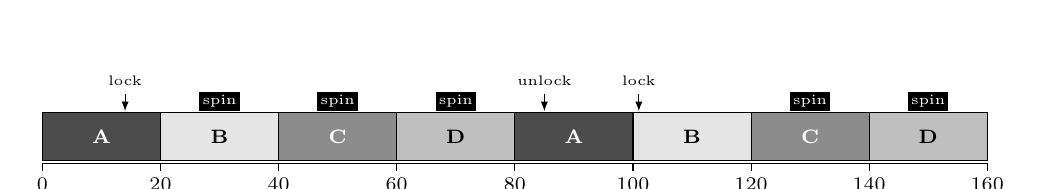
\begin{tikzpicture}[tl]
  \blk{0}{20}{A}{thA}{white}    \blk{20}{40}{B}{thB}{black}
  \blk{40}{60}{C}{thC}{white}   \blk{60}{80}{D}{thD}{black}
  \blk{80}{100}{A}{thA}{white}  \blk{100}{120}{B}{thB}{black}
  \blk{120}{140}{C}{thC}{white} \blk{140}{160}{D}{thD}{black}
  \foreach \s in {20,40,60,120,140} { \spin{\s}{\s+20} }
  \ev{14}{lock} \ev{85}{unlock} \ev{101}{lock}
  \taxis
\end{tikzpicture}
\end{center}

A takes the lock at time \(\approx 14\). B, C and D are then scheduled one
after another and each spins for a full slice (20--80) while A, the only
thread that can make progress, waits in the ready queue. A unlocks at
\(\approx 85\); B finally gets the lock at \(\approx 101\); C and D spin
again. \textbf{The CPU scheduler may run B instead of A even though B is
waiting for A.}

\keepspace{24\baselineskip}
\subsection{Ticket lock with \texttt{yield()}}

\begin{lstlisting}
typedef struct __lock_t {
        int ticket;
        int turn;
} lock_t;

void lock_init(lock_t *lock) {
        lock->ticket = 0;
        lock->turn = 0;
}

void acquire(lock_t *lock) {
    int myturn = FAA(&lock->ticket);
    while(lock->turn != myturn)
        yield();
}

void release (lock_t *lock) {
    FAA(&lock->turn);
}
\end{lstlisting}

Instead of spinning, a waiter that finds it is not its turn calls
\texttt{yield()}: it gives up the CPU right away and goes back to the ready
queue.

\subsection{Yield instead of spin}

\begin{center}
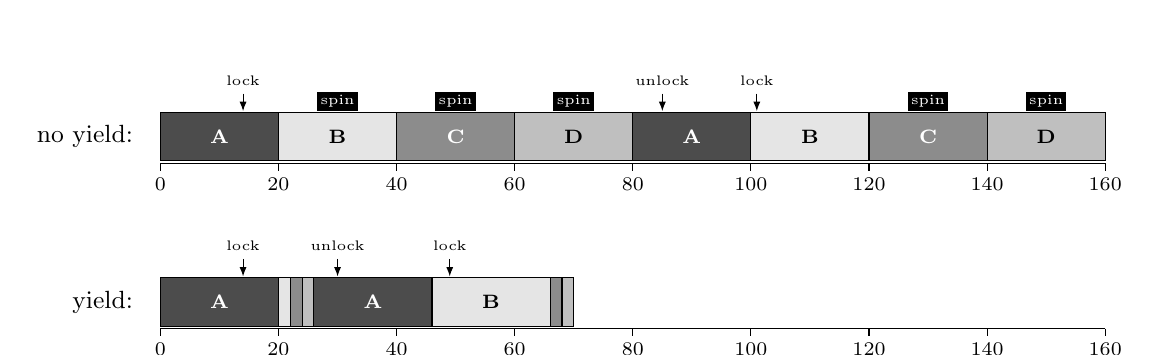
\begin{tikzpicture}[tl]
  \node[anchor=east, font=\small] at (-3,0.5) {no yield:};
  \blk{0}{20}{A}{thA}{white}    \blk{20}{40}{B}{thB}{black}
  \blk{40}{60}{C}{thC}{white}   \blk{60}{80}{D}{thD}{black}
  \blk{80}{100}{A}{thA}{white}  \blk{100}{120}{B}{thB}{black}
  \blk{120}{140}{C}{thC}{white} \blk{140}{160}{D}{thD}{black}
  \foreach \s in {20,40,60,120,140} { \spin{\s}{\s+20} }
  \ev{14}{lock} \ev{85}{unlock} \ev{101}{lock}
  \taxis
  \begin{scope}[yshift=-2.1cm]
  \node[anchor=east, font=\small] at (-3,0.5) {yield:};
  \blk{0}{20}{A}{thA}{white}
  \draw[thB] (20,0) rectangle (22,1); \draw[thC] (22,0) rectangle (24,1); \draw[thD] (24,0) rectangle (26,1);
  \blk{26}{46}{A}{thA}{white}  \blk{46}{66}{B}{thB}{black}
  \draw[thC] (66,0) rectangle (68,1); \draw[thD] (68,0) rectangle (70,1);
  \ev{14}{lock} \ev{30}{unlock} \ev{49}{lock}
  \taxis
  \end{scope}
\end{tikzpicture}
\end{center}

With \texttt{yield()}, B, C and D each run only for a sliver (just long
enough to check and yield), so A gets the CPU back almost immediately,
unlocks at \(\approx 30\), and B takes the lock at \(\approx 49\) instead of
\(\approx 101\).

\begin{keybox}[Waste]
\begin{itemize}
  \item Without yield: \(O(\text{threads} \times \text{time\_slice})\).
  \item With yield: \(O(\text{threads} \times \text{context\_switch})\).
\end{itemize}
So even with yield, spinning is slow with \textbf{high thread contention}:
every waiting thread still gets scheduled and pays a context switch just to
find out it must wait.

\textbf{Next improvement:} block and put the thread on a \textbf{waiting
queue} instead of spinning.
\end{keybox}

% ===========================================================================
\section{Lock implementation: block when waiting}
% ===========================================================================

The lock implementation \textbf{removes waiting threads from the scheduler's
ready queue} (e.g.\ with \texttt{park()} and \texttt{unpark()}). The
\textbf{scheduler runs any thread that is ready}. Good separation of
concerns: the lock decides who may run, and the scheduler only sees threads
that can actually make progress.

Why this is needed: spinning and yielding both \textbf{leave too much to
chance}. The scheduler still picks the next thread, and a bad pick runs a
thread that can only spin or immediately yield. That wastes time, and with
a plain test-and-set lock plus \texttt{yield()}, a thread can even starve,
yielding forever while others keep re-entering. The queue lets the
\emph{lock} decide who gets it next.

\begin{itemize}
  \item \texttt{park()}: put the calling thread to sleep (it leaves the
        ready queue).
  \item \texttt{unpark(tid)}: wake thread \texttt{tid} (it goes back to the
        ready queue).
\end{itemize}

\subsection{Walkthrough (animation on the slides)}

Four threads A, B, C, D share one CPU. Each row is one slide of the
animation; the state is shown \emph{after} the event.

\begin{center}
\renewcommand{\arraystretch}{1.08}
\small
\begin{tabular}{@{}clllp{5.4cm}@{}}
  \toprule
  \textbf{Time} & \textbf{RUNNABLE} & \textbf{RUNNING} & \textbf{WAITING} & \textbf{Event} \\
  \midrule
  --       & A, B, C, D & \textless empty\textgreater & \textless empty\textgreater & start \\
  0        & B, C, D & A & \textless empty\textgreater & A runs, takes the \textbf{lock} \\
  20       & C, D, A & B & \textless empty\textgreater & slice ends, B runs \\
  \(\approx\)35 & C, D, A & -- & B & B \textbf{tries lock}, \textbf{sleeps} (parked) \\
  35       & D, A & C & B & C runs (no lock needed) \\
  55       & A, C & D & B & D runs \\
  \(\approx\)72 & A, C & -- & B, D & D tries lock, sleeps \\
  72       & C & A & B, D & A runs \\
  92       & A & C & B, D & C runs \\
  112      & C & A & B, D & A runs \\
  \(\approx\)118 & B, C & A & D & A \textbf{unlocks}: B woken (back to RUNNABLE) \\
  132      & C, A & B & D & B runs and now holds the \textbf{lock} \\
  \bottomrule
\end{tabular}
\end{center}

\begin{center}
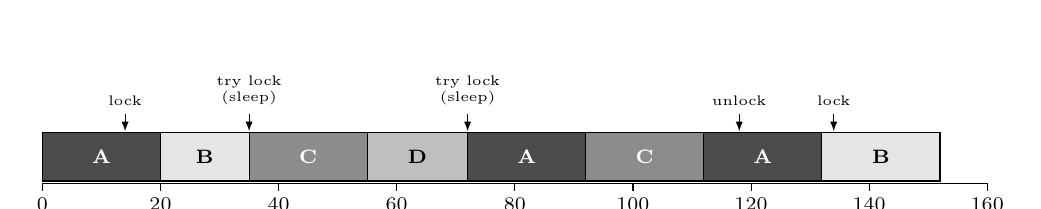
\begin{tikzpicture}[tl]
  \blk{0}{20}{A}{thA}{white}   \blk{20}{35}{B}{thB}{black}
  \blk{35}{55}{C}{thC}{white}  \blk{55}{72}{D}{thD}{black}
  \blk{72}{92}{A}{thA}{white}  \blk{92}{112}{C}{thC}{white}
  \blk{112}{132}{A}{thA}{white}\blk{132}{152}{B}{thB}{black}
  \ev{14}{lock} \ev{35}{try lock\\(sleep)} \ev{72}{try lock\\(sleep)}
  \ev{118}{unlock} \ev{134}{lock}
  \taxis
\end{tikzpicture}
\end{center}

Compare with the spinning timelines: B and D are \textbf{never scheduled}
while they cannot make progress. No time slice is wasted on spinning; the
CPU goes to A and C, which can do useful work.

\keepspace{30\baselineskip}
\subsection{Implementation with a guard and a queue}

\begin{lstlisting}
typedef struct {
   bool lock = false;
   bool guard = false;
   queue_t q;
} LockT;

void acquire(LockT *l) {
   while (TAS(&l->guard, true));
   if (l->lock) {
       qadd(l->q, tid);
       l->guard = false;
       park();     // blocked
   } else {
       l->lock = true;
       l->guard = false;
   }
}

void release(LockT *l) {
   while (TAS(&l->guard, true));
   if (qempty(l->q)) l->lock=false;
   else unpark(qremove(l->q));
   l->guard = false;
}
\end{lstlisting}

(\texttt{TAS} = test-and-set, i.e.\ \texttt{xchg}.)

\begin{solbox}[The slide's questions]
\begin{enumerate}[(a)]
  \item \textbf{Why is \texttt{guard} used?} \texttt{lock} and the queue
        \texttt{q} are themselves shared data that several threads update in
        \texttt{acquire} and \texttt{release}. \texttt{guard} is a small
        spinlock that makes those few updates (check \texttt{lock}, add to /
        remove from \texttt{q}) a critical section.
  \item \textbf{Why is it okay to spin on \texttt{guard}?} \texttt{guard} is
        held only for the handful of instructions inside \texttt{acquire} /
        \texttt{release}, never for the user's critical section. So the
        spin is very short. Threads waiting for the real lock sleep.
  \item \textbf{In \texttt{release()}, why not set \texttt{lock = false}
        when unparking?} The lock is \textbf{handed directly} to the woken
        thread. It returns from \texttt{park()} already owning the lock and
        does not re-check \texttt{lock}; it does not hold \texttt{guard} at
        that point, so it could not safely set \texttt{lock} itself. If
        \texttt{release} set \texttt{lock = false}, a third thread could grab
        the lock in the meantime and then two threads would be inside the
        critical section.
  \item \textbf{What is the race condition?} See below.
\end{enumerate}
\end{solbox}

\subsection{The race condition}

\begin{center}
\renewcommand{\arraystretch}{1.12}
\begin{tabular}{@{}ll@{}}
  \toprule
  \textbf{Thread 1} (in lock) & \textbf{Thread 2} (in unlock) \\
  \midrule
  \texttt{if (l->lock) \{} & \\
  \texttt{\ \ \ qadd(l->q, tid);} & \\
  \texttt{\ \ \ l->guard = false;} & \\
  & \texttt{while (TAS(\&l->guard, true));} \\
  & \texttt{if (qempty(l->q)) // false!!} \\
  & \texttt{else unpark(qremove(l->q));} \\
  & \texttt{l->guard = false;} \\
  \texttt{\ \ \ park(); \ \ // block} & \\
  \bottomrule
\end{tabular}
\end{center}

\begin{warnbox}[Problem: guard not held when calling \texttt{park()}]
The unlocking thread may \texttt{unpark()} \textbf{before} the other thread
calls \texttt{park()}. The wakeup is delivered to a thread that is not
asleep yet and is lost. Thread 1 then parks with the lock already handed to
it, and may sleep forever.
\end{warnbox}

\keepspace{27\baselineskip}
\subsection{Final correct lock}

\begin{lstlisting}
Typedef struct {
   bool lock = false;
   bool guard = false;
   queue_t q;
} LockT;

void acquire(LockT *l) {
   while (TAS(&l->guard, true));
   if (l->lock) {
       qadd(l->q, tid);
       setpark(); // notify of plan
       l->guard = false;
       park(); // unless unpark()
   } else {
       l->lock = true;
       l->guard = false;
   }
}

void release(LockT *l) {
   while (TAS(&l->guard, true));
   if (qempty(l->q)) l->lock=false;
   else unpark(qremove(l->q));
   l->guard = false;
}
\end{lstlisting}

\keepspace{8\baselineskip}
\begin{keybox}[\texttt{setpark()} fixes the race condition]
\texttt{setpark()} tells the OS ``I am about to park.'' If another thread
calls \texttt{unpark()} on this thread between \texttt{setpark()} and
\texttt{park()}, the later \texttt{park()} returns immediately instead of
sleeping. The wakeup is no longer lost.

The race exists because releasing \texttt{guard} and parking are two
separate steps. Another possible fix is to pass \texttt{guard} into the
kernel, which then releases it and puts the thread to sleep atomically.
\end{keybox}

% ===========================================================================
\section{Spin-waiting vs.\ blocking}
% ===========================================================================

Each approach is better under different circumstances.

\begin{itemize}
  \item \textbf{Uniprocessor}
    \begin{itemize}
      \item Waiting process is scheduled \(\Rightarrow\) the process holding
            the lock isn't.
      \item So the waiting process should \textbf{always relinquish} the
            processor.
      \item Associate a queue of waiters with each lock (as in the previous
            implementation).
    \end{itemize}
  \item \textbf{Multiprocessor}
    \begin{itemize}
      \item Waiting process is scheduled \(\Rightarrow\) the process holding
            the lock \emph{might} be (on another CPU).
      \item Spin or block depends on how long, \(t\), before the lock is
            released:
        \begin{itemize}
          \item lock released quickly \(\Rightarrow\) \textbf{spin-wait};
          \item lock released slowly \(\Rightarrow\) \textbf{block}.
        \end{itemize}
      \item ``Quick'' and ``slow'' are relative to the
            \textbf{context-switch cost}, \(C\).
    \end{itemize}
\end{itemize}

\keepspace{16\baselineskip}
\subsection{When to spin-wait? When to block?}

If we know how long, \(t\), before the lock is released, we can determine
the optimal behaviour.

\begin{center}
\renewcommand{\arraystretch}{1.2}
\begin{tabular}{@{}ll@{}}
  \toprule
  \textbf{Question} & \textbf{Answer} \\
  \midrule
  How much CPU time is wasted when spin-waiting? & \(t\) \\
  How much is wasted when blocking? & \(C\) \\
  Best action when \(t < C\)? & \textbf{spin-wait} \\
  Best action when \(t > C\)? & \textbf{block} \\
  \bottomrule
\end{tabular}
\end{center}

\begin{warnbox}[Problem]
This requires \textbf{knowledge of the future}; it is too much overhead to
do any special prediction.
\end{warnbox}

\keepspace{16\baselineskip}
% ===========================================================================
\section{Summary}
% ===========================================================================

\begin{center}
\renewcommand{\arraystretch}{1.2}
\small
\begin{tabularx}{\textwidth}{@{}lX@{}}
  \toprule
  \textbf{Approach} & \textbf{Verdict} \\
  \midrule
  Disable interrupts & Works only on uniprocessors; a thread can hog the CPU;
                       OS misses interrupts. \\
  Single flag (loads/stores) & Broken: test and set are not atomic, both
                       threads can enter. \\
  Peterson's algorithm & Correct for two threads with only loads and stores. \\
  \texttt{xchg} / test-and-set & Correct spinlock (mutual exclusion), but
                       unfair. \\
  Compare-and-swap & Same spinlock as \texttt{xchg}, using \texttt{CAS(flag, 0, 1)}. \\
  Ticket lock (fetch-and-add) & Fair: threads served in order of arrival. \\
  Ticket lock + \texttt{yield()} & Waste drops from
                       \(O(\text{threads}\times\text{time\_slice})\) to
                       \(O(\text{threads}\times\text{context\_switch})\). \\
  Queue + \texttt{park}/\texttt{unpark} & Waiters sleep; \texttt{guard}
                       protects lock state; \texttt{setpark()} fixes the
                       wakeup race. \\
  \bottomrule
\end{tabularx}
\end{center}

\begin{keybox}[Spin or block?]
Spin when the expected wait \(t\) is shorter than a context switch \(C\)
(multiprocessor, short critical sections); block otherwise, and always
block on a uniprocessor.
\end{keybox}

\end{document}
